\documentclass[12pt]{article}%
\usepackage{amsmath,amssymb,amsthm,amsfonts}
\usepackage{wasysym}
\usepackage{graphicx}
\usepackage[dvipsnames]{xcolor}
\usepackage{stackengine}
\def\stackalignment{l}
\usepackage[colorlinks]{hyperref}
\usepackage{tikz}
\usepackage[export]{adjustbox}

\ProvidesPackage{commands}

%---Packages---%
\usepackage{amssymb, fullpage, amsmath, esint}
\usepackage{graphicx}
\usepackage{empheq}
\usepackage{float}
\usepackage{listings}
\usepackage{color}
\usepackage{caption}
\usepackage{subcaption}

\usepackage{matlab-prettifier}

%---Environments---%
\newtheorem{problem}{Problem}
\newenvironment{solution}[1][\it{Solution}]{\textbf{#1. } }{$\square$}

%---Style---%
\graphicspath{ {./} }
\allowdisplaybreaks
\pagestyle{empty}
%\numberwithin{equation}{subsection}


%---Definitions---%
\def\Z{{\mathbb Z}}
\def\Q{{\mathbb Q}}
\def\C{{\mathbb C}}
\def\R{{\mathbb R}}
\def\N{{\mathbb N}}
\def\eps{{\epsilon}}
\def\O{{\mathcal{O}}}
\def\F{{\mathcal{F}}}
\def\ointcc{{\ointctrclockwise}} %counter clockwise contour integral
\def\ointc{{\ointclockwise}} %clockwise contour integral
\def\and{{~\text{and}~}} %and


%dash integral 
\def\Xint#1{\mathchoice
   {\XXint\displaystyle\textstyle{#1}}%
   {\XXint\textstyle\scriptstyle{#1}}%
   {\XXint\scriptstyle\scriptscriptstyle{#1}}%
   {\XXint\scriptscriptstyle\scriptscriptstyle{#1}}%
   \!\int}
\def\XXint#1#2#3{{\setbox0=\hbox{$#1{#2#3}{\int}$}
     \vcenter{\hbox{$#2#3$}}\kern-.5\wd0}}
\def\ddashint{\Xint=}
\def\dashint{\Xint-}


%---Commands---%
\newcommand{\floor}[1]{{\left\lfloor#1\right\rfloor}} % Floor function
\newcommand{\ceil}[1]{{\left\lceil#1\right\rceil}} % Ceiling function
\newcommand{\paren}[1]{{\left(#1\right)}} % Parentheses ()
\newcommand{\brac}[1]{{\left\{#1\right\}}} % Curly braces {}
\newcommand{\braces}[1]{{\left[#1\right]}} % Braces []
\newcommand{\abrac}[1]{{\left\langle#1\right\rangle}} % Angle Braces <>
\newcommand{\abs}[1]{{\left|#1\right|}} % Absolute value
\newcommand{\norm}[1]{{\left\|#1\right\|}} % Norm
\newcommand{\eval}[2]{\right|_{#1}^{#2}} % Evaluate
\newcommand{\pp}[2]{\frac{\partial #1}{\partial #2}} % Partial of 1 wrt 2
\newcommand{\ppn}[3]{\frac{\partial^{#1} #2}{\partial #3^{#1}}} % nth Partial of 1 wrt 2
\newcommand{\dd}[2]{\frac{\mathrm{d} #1}{\mathrm{d} #2}} % Partial of 1 wrt 2
\newcommand{\ddn}[3]{\frac{\mathrm{d}^{#1} #2}{\mathrm{d} #3^{#1}}} % nth Partial of 1 wrt 2
\newcommand\fullref[1]{Eq.~(\ref*{#1})} % Eq.()
\newcommand\dt[1]{\mathrm{d}#1} %dt

%boxed solution with spacing 0.5cm around equations
\setlength\fboxsep{0.5cm}
\newcommand*\widefbox[1]{\fbox{#1}}


%MATLAB formatting
\definecolor{mygreen}{rgb}{0,0.6,0}
\definecolor{mygreen}{RGB}{28,172,0} % color values Red, Green, Blue
\definecolor{mylilas}{RGB}{170,55,241}
\definecolor{light-gray}{gray}{0.95} %the shade of grey that stack exchange uses
\lstset{ 
    backgroundcolor=\color{light-gray},
}
\lstset{language=Matlab,%
    %basicstyle=\color{red},
    breaklines=true,%
    morekeywords={matlab2tikz},
    keywordstyle=\color{blue},%
    morekeywords=[2]{1}, keywordstyle=[2]{\color{black}},
    identifierstyle=\color{black},%
    stringstyle=\color{mylilas},
    commentstyle=\color{mygreen},%
    showstringspaces=false,%without this there will be a symbol in the places where there is a space
    numbers=left,%
    numberstyle={\tiny \color{black}},% size of the numbers
    numbersep=9pt, % this defines how far the numbers are from the text
    emph=[1]{for,end,break},emphstyle=[1]\color{red}, %some words to emphasise
    %emph=[2]{word1,word2}, emphstyle=[2]{style},    
}

%\usepackage{geometry}
%\geometry{top = 0.9in}
\usepackage{appendix}


\renewcommand{\S}{\mathbb{S}^1}
\renewcommand{\Re}{\text{Re}}
\newcommand{\ea}{\textit{et al. }}
\renewcommand{\epsilon}{\varepsilon}
\renewcommand{\th}{\text{th}}
\newcommand{\sgn}{\operatorname{sgn}}

\renewcommand{\setminus}{\smallsetminus}

\newtheorem{thm}{Theorem}
\newtheorem{lemma}{Lemma}

\definecolor{red}{rgb}{0.8500, 0.3250, 0.0980}
\definecolor{green}{rgb}{0.4660, 0.6740, 0.1880}
\definecolor{yellow}{rgb}{0.9290, 0.6940, 0.1250}
\definecolor{blue}{rgb}{0, 0.4470, 0.7410}


\begin{document}

\title{Coding Project:  MNIST Classification Problem}

\author{Marvyn Bailly}
\date{}

\maketitle


\begin{abstract}
In this coding project, we explore the classification problem for the MNSIT dataset. Specifically, we will classify $1$s and $7$s from the dataset. We begin by implementing the Levenberg-Marquardt, Stochastic Gradient Descent, Stochastic Nesterov, and Stochastic Adams methods in MATLAB. We first observe the accuracy of the Levenberg-Marquardt method and conclude by comparing the effectiveness of the stochastic methods. 
\end{abstract}

\section{classification Problem}
Working from the classic MNIST dataset, we wish to train an algorithm to classify $1$'s and $7$'s. We will use a dividing surface that separates the images containing $1$ from those containing $7$. A sample of $1$'s and $7$'s from the training set is shown in Fig \ref{fig1}. Each image is a point in $\R^{400}$, so we will use PCA to reduce the dimensionality of the problem. Rather than using a hyperplane to separate the data, we aim to find an optimal quadratic hypersurface with Tikhonov regularization. That is, we wish to find a quadratic hypersurface of the form
\begin{equation*}
    x^\top W x + v^\top x + b.
\end{equation*}
This gives the quadratic test function is of the form
\begin{equation}\label{equation 3}
    q(x_j;\mathbf{w}) := y_j (x^\top W x + v^\top x + b).
\end{equation}
Similarly, we define the loss function as
\begin{equation}\label{equation 4}
    f(\mathbf{w}) = \frac{1}{n} \sum_{j=1}^n \log(1 + e^{-q(x_j ; \mathbf{w})}) + \frac{\lambda}{2}\|\mathbf{w}\|^2.
\end{equation}
Here $\mathbf{w}$ denotes the $d^2 + d + 1$ dimensional vector of coefficients of $\brac{W,v,b}$. Finally, we fit the loss function to fit the framework of the nonlinear least squares problem:
\begin{equation}\label{equation 5}
    f(\mathbf{w}) = \frac{1}{2} \sum_{j=1}^n (r_j(\mathbf{w}))^2, \quad r_j(\mathbf{w}) = \log(1  + e^{-q(x_j; \mathbf{w})}).
\end{equation}
We also note that there are $6742$ $1$'s and $6265$ $7$'s in training data
There are $1135$ $1$'s and $1028$ $7$'s in test data.

\begin{figure}[H]
    \begin{subfigure}[b]{0.5\linewidth}
        \centering
        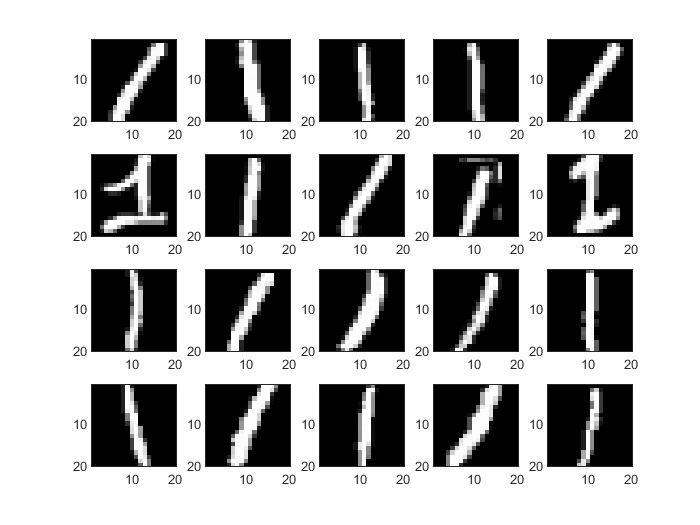
\includegraphics[width=\linewidth]{images/sample1.png}
        \caption{}
        \label{fig1:a}
        \vspace{4ex}
    \end{subfigure}%%
    \begin{subfigure}[b]{0.5\linewidth}
        \centering
        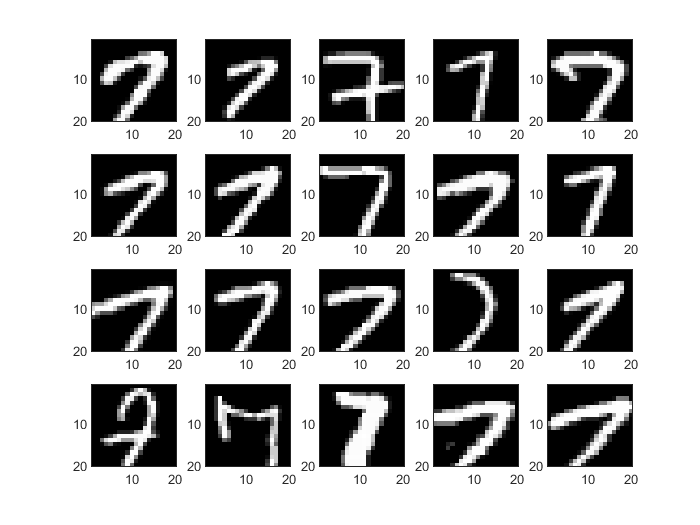
\includegraphics[width=\linewidth]{images/sample7.png}
        \caption{}
        \label{fig1:b}
        \vspace{4ex}
    \end{subfigure}
    \caption{Samples of 20-by-20 images of $1's$ (a) and $7$'s (b) from MNIST.}
    \label{fig1}
\end{figure}

\section{Methods}
To find an appropriate amount of PCAs to use, we plot the singular values of the data set, as seen in Fig. \ref{figpca}. We see that using around $20$ singular values is reasonable.

\begin{figure}[H]
    \centering
    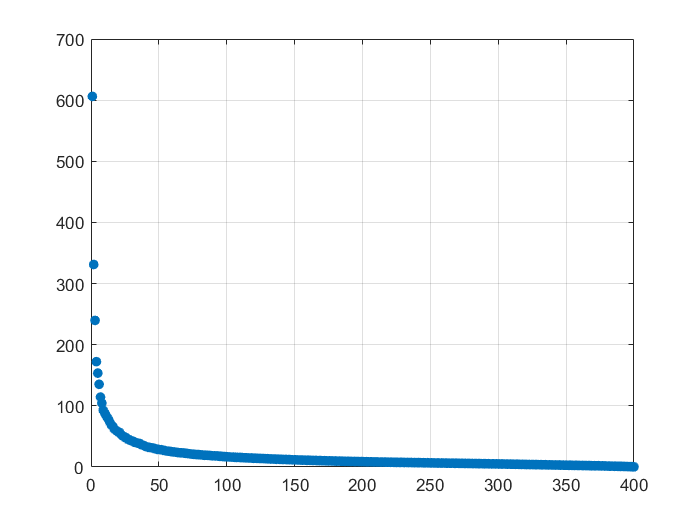
\includegraphics[width=0.5\textwidth,height=\textwidth,keepaspectratio]{images/PCA.png}
    \caption{Plot of the singular values of the dataset.}
    \label{figpca}
\end{figure}

\subsection{Levenberg-Marquardt}
Setting the number of PCAs to twenty, we wish to find the optimal quadratic dividing surface of \fullref{equation 3} using the Levenberg-Marquardt method. We implement the method in MatLab (see \ref{LM-code} for code) where we use the regularization 
\begin{equation*}
    J^\top J + I \cdot 10^{-6},
\end{equation*}
to avoid issues inverting the matrix $J^\top J$.  

\subsection{Stochastic Optimizers}
Next, we wish to use the following three stochastic optimizers to minimize the loss function \ref{equation 5} and the final optimal dividing quadratic hypersurface. We implement the Stochastic Gradient Descent (see \ref{SGC-code} for code) where we will use various batch sizes and stepsize decreasing methods, the Stochastic Nesterov method (see \ref{nesterov-code}) where we will use various batch sizes, and the deterministic version of Stochastic Adams method (see \ref{adams-code} for code.).


\section{Results}
\subsection{Levenberg-Marquardt}
Running the Levenberg-Marquardt method for $20$ PCAs, a tolerance of $10^{-3}$, a trust region max of $1$ and min of $10^{-14}$; $\rho_\text{bad} = 0.25$ and $\rho_\text{good} = 0.75$; and $\eta = 0.01$, we get that the method converges after $35$ iterations. The hypersurface classifies $2152$ of the numbers correctly while getting $11$, giving an accuracy of $99.4$ percent. A plot of the gradient and the function value at each iteration can be seen in Figure \ref{LM}. Setting the number of PCAs to $3$, we can visualize the optimal hypersurface as seen in Figure 

\begin{figure}[H]
    \begin{subfigure}[b]{0.5\linewidth}
        \centering
        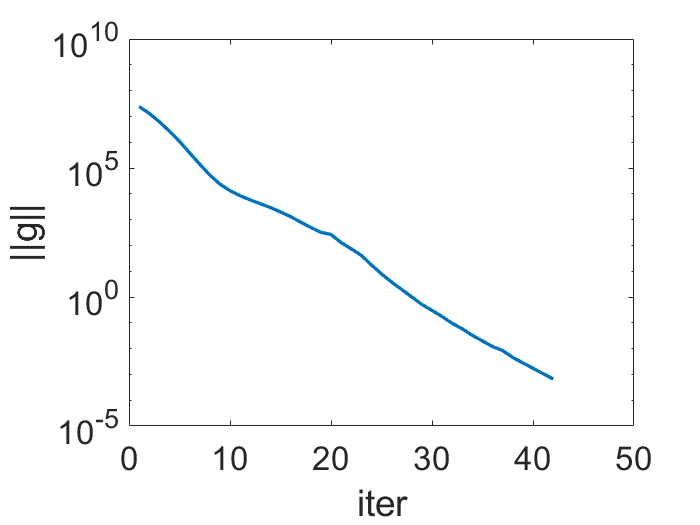
\includegraphics[width=\linewidth]{images/LM-gnorm.png}
        \caption{}
        \label{LM:a}
        \vspace{4ex}
    \end{subfigure}%%
    \begin{subfigure}[b]{0.5\linewidth}
        \centering
        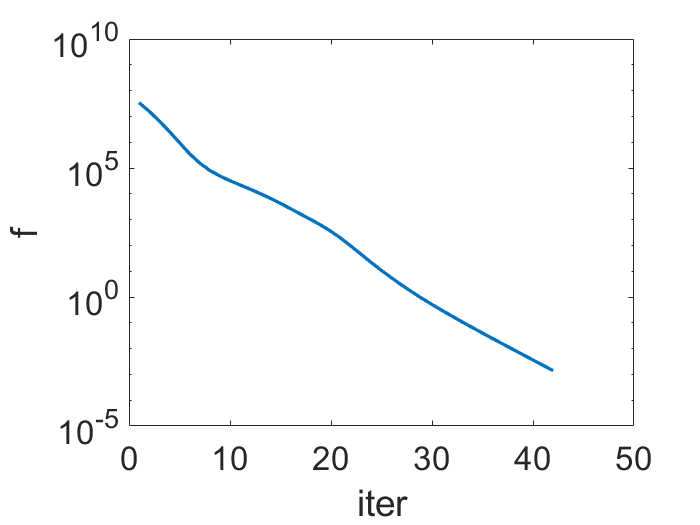
\includegraphics[width=\linewidth]{images/LM-f.png}
        \caption{}
        \label{LM:b}
        \vspace{4ex}
    \end{subfigure}
    \caption{The plot of the gradient (a) and the function value (b) at each iteration using the Levenberg-Marquardt method.}
    \label{LM}
\end{figure}

\begin{figure}[H]
    \centering
    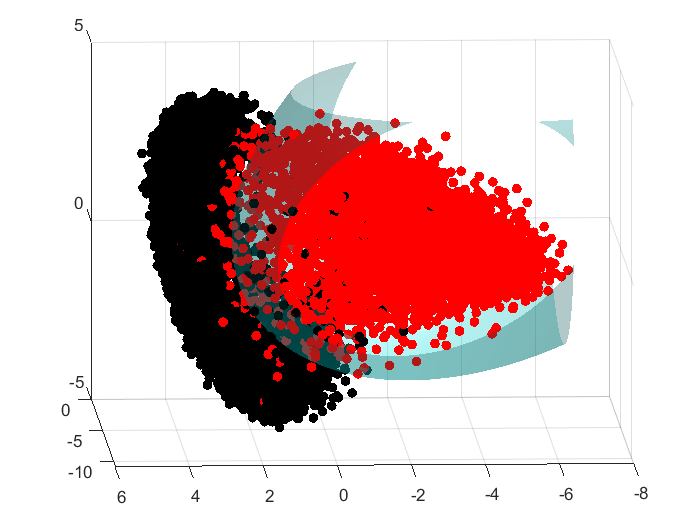
\includegraphics[width=0.5\textwidth,height=\textwidth,keepaspectratio]{images/LM-hypersurface.png}
    \caption{Visualization of the optimal hypersurface found by the Levenberg-Marquardt method. Here black data points correspond to the $1$ labels, red corresponds to $7$ labels, and blue shows the hypersurface.}
    \label{fig}
\end{figure}


\subsection{Stochastic Optimizers}
Next, we will use stochastic methods to minimize the loss function Equation \ref{equation 4} and find the optimal dividing quadratic hypersurface. We first look at the Stochastic Gradient Descent method and experiment with various batch sizes and step-size decreasing methods. The various step-size decreasing methods we will try are the following: keeping $\alpha$ fixed, starting $\alpha =0.3$ and updating $\alpha = 0.999\alpha$ on each iteration; starting $\alpha = 0.3$ and updating $\alpha = 0.3/k^2$; and starting $\alpha = 0.3$ and updating $\alpha = 0.3/2^k$. For all of the Stochastic methods, we will fix the number of max iterations to $3000$ and test batch sizes of $10,100,1000$. This means that for each batch size, there are a fixed number of epochs. The results for Stochastic Gradient Descent can be seen in Table \ref{CG-table}. Notice that the highest percentage of accuracy is given $99.3$ percent and is achieved with a batch size of $1000$ and holding $\alpha = 0.3$ fixed. This is closely followed by $99.2$ percent accuracy when the batch size is $100$ and $\alpha =0.3$ is fixed and when the batch size is $10$ and $\alpha = 0.999 \cdot \alpha$ is the update method. The plot of the norm of the gradient and function value over the epochs can be seen in Figure \ref{CG} where we can see that the average function value decreases over the epoch with decreasingly small spikes. We also note that the norm of the gradient stays around $10^{-1}$ and $10^{-2}$.

\begin{table}[h!]
    \centering
    \begin{tabular}{c|c|c|c}
        accuracy&  bsz = 10& bsz = 100 &  bsz = 1000  \\ \hline
        $\alpha = 0.3$&  98.6\% &  99.2\%&  99.3\%  \\
        $\alpha = 0.01$&  98.3\% &  98.2\%&  98.5\%  \\
        $\alpha = 0.999 \cdot \alpha$&  99.2\%&  99.0\%&  98.6\% \\
        $\alpha = 0.3/k^2$&  86.2\%&  93.2\%&   89.3\%\\
        $\alpha = 0.3/2^k$&  71.5\%&  89.3\%&   88.2\%\\
    \end{tabular}
    \caption{}
    \label{CG-table}
\end{table}

\begin{figure}[H]
    \begin{subfigure}[b]{0.5\linewidth}
        \centering
        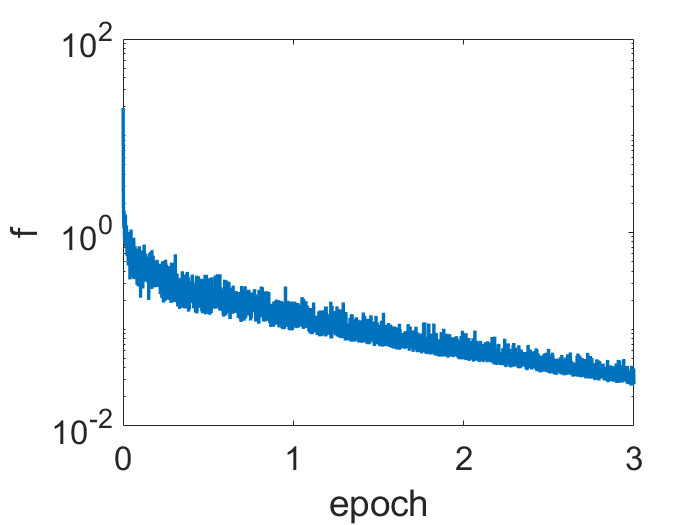
\includegraphics[width=\linewidth]{images/sg-f.png}
        \caption{}
        \label{CG:a}
        \vspace{4ex}
    \end{subfigure}%%
    \begin{subfigure}[b]{0.5\linewidth}
        \centering
        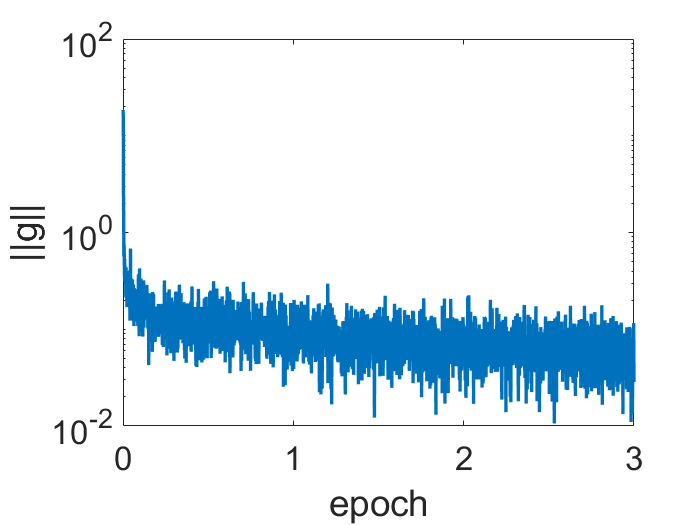
\includegraphics[width=\linewidth]{images/sg-g.png}
        \caption{}
        \label{CG:b}
        \vspace{4ex}
    \end{subfigure}
    \caption{Plot of the function value (a) and norm of the gradient (b) compared to the epoch using Stochastic Gradient Descent with batch size of $1000$ and $\alpha = 0.3$ fixed.}
    \label{CG}
\end{figure}

Next, we look at the deterministic Stochastic Nesterov method and experiment with various batch sizes. The results can be seen in Table \ref{nesterov-table}. Notice that the best accuracy is achieved at $99.3\%$ when using a batch size of $1000$ and is closely followed by $99.2\%$ when using a batch size of $100$. The plot of the norm of the gradient and function value over the epochs can be seen in Figure \ref{nesterov} where we can see that the average function value decreases until it reaches around $10^{-2}$. We also note that the norm of the gradient stays around $10^{-1}$ and $10^{-2}$.

\begin{table}[h!]
    \centering
    \begin{tabular}{c|c|c|c}
        &  bsz = 10& bsz = 100 &  bsz = 1000  \\ \hline
        accuracy &  98.5\% &  99.2\%&  99.3\%  \\
    \end{tabular}
    \caption{}
    \label{nesterov-table}
\end{table}
\begin{figure}[H]
    \begin{subfigure}[b]{0.5\linewidth}
        \centering
        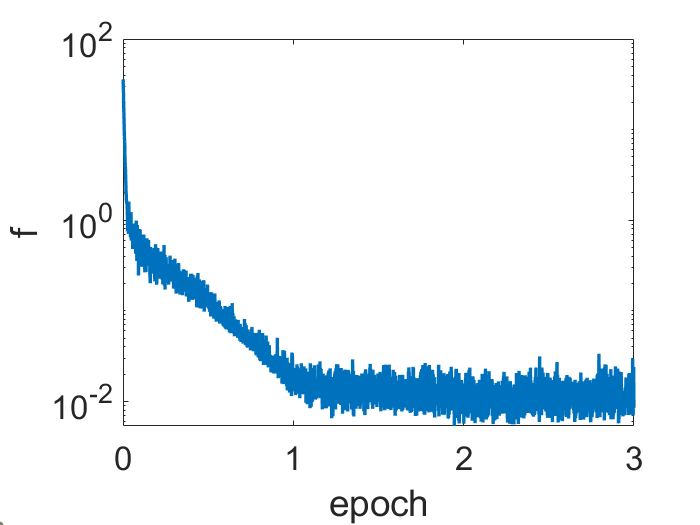
\includegraphics[width=\linewidth]{images/nest-f.png}
        \caption{}
        \label{nesterov:a}
        \vspace{4ex}
    \end{subfigure}%%
    \begin{subfigure}[b]{0.5\linewidth}
        \centering
        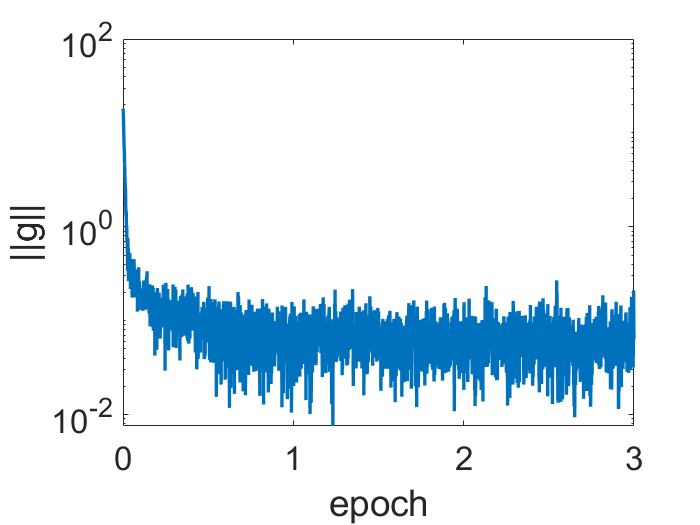
\includegraphics[width=\linewidth]{images/nest-g.png}
        \caption{}
        \label{nesterov:b}
        \vspace{4ex}
    \end{subfigure}
    \caption{Plot of the function value (a) and norm of the gradient (b) compared to the epoch using deterministic Stochastic Nesterov method with batch size of $1000$.}
    \label{nesterov}
\end{figure}

Finally, we look at the Stochastic Adams method and experiment with various batch sizes. Note that we use the standard settings $\beta_1 = 0.9$, $\beta_2 = 0.999$, $\alpha = 0.001$, and $\eps = 10^{-8}$. The results can be seen in Table \ref{adams-table}. Once again, the best accuracy is achieved at $98.3\%$ when using a batch size of $1000$ and is closely followed by $98.2\%$ when using a batch size of $100$. The plot of the norm of the gradient and function value over the epochs can be seen in Figure \ref{Adams} where we can see that the average function value decreases and the spikes seem well maintained. The same holds for the gradient. 

\begin{table}[h!]
    \centering
    \begin{tabular}{c|c|c|c}
        &  bsz = 10& bsz = 100 &  bsz = 1000  \\ \hline
        accuracy&  97.3\% &  98.2\%&  98.7\%  \\
    \end{tabular}
    \caption{}
    \label{adams-table}
\end{table}
\begin{figure}[H]
    \begin{subfigure}[b]{0.5\linewidth}
        \centering
        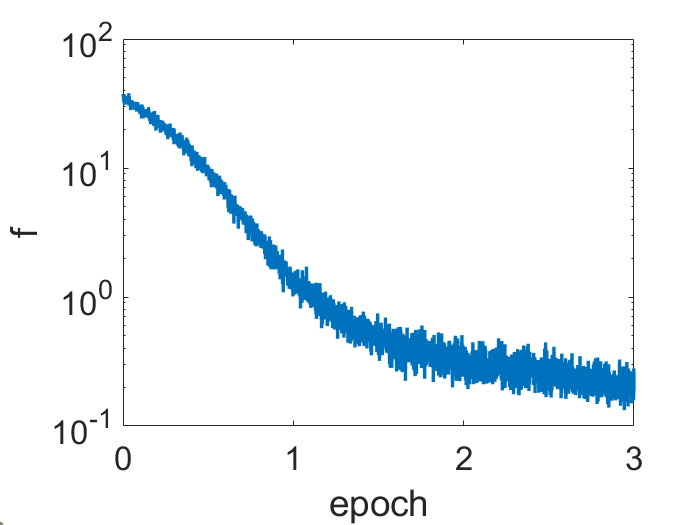
\includegraphics[width=\linewidth]{images/adams-f.png}
        \caption{}
        \label{Adams:a}
        \vspace{4ex}
    \end{subfigure}%%
    \begin{subfigure}[b]{0.5\linewidth}
        \centering
        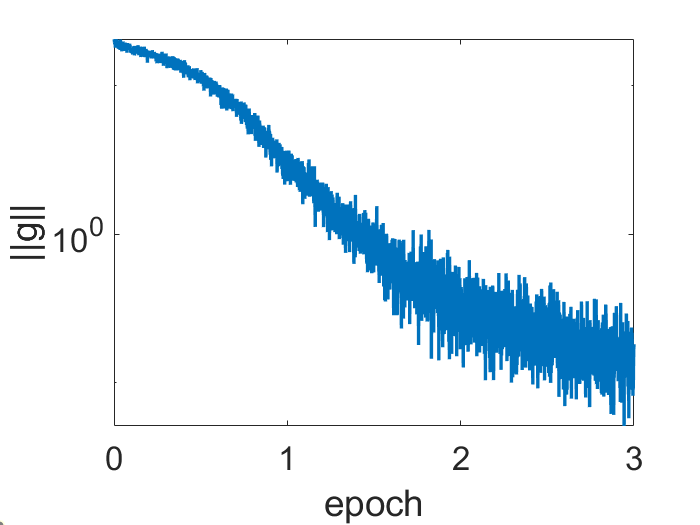
\includegraphics[width=\linewidth]{images/adams-g.png}
        \caption{}
        \label{Adams:b}
        \vspace{4ex}
    \end{subfigure}
    \caption{Plot of the function value (a) and norm of the gradient (b) compared to the epoch using Stochastic Adams method with batch size of $1000$.}
    \label{Adams}
\end{figure}




\section{Conclusion}
In conclusion, we see that the Levenberg-Marquardt method achieves the best accuracy of $99.4$ percent. Closely following are the Stochastic Gradient Descent with $99.3$ percent accuracy when using a batch size of $1000$, and the Stochastic Adams achieves $98.7$. Out of the Stochastic methods, the Stochastic Gradient and Nesterov are able to achieve the same accuracy but it is worth noting that the graphs of their function values and norm of the gradients (see Figures \ref{CG} and \ref{nesterov}) show that the level of chaos in the spikes is better contained when using Stochastic gradient descent which may or may not be favorable. We also note that the function values for the Nesterov method approach $10^{-2}$ in fewer epochs than gradient descent. Since both methods hover around $10^{-2}$, this suggests that the Nesterov method has the best accuracy in the fewest iterations. On the other hand, looking at the graph of stochastic gradient descent, it appears that it could achieve higher accuracy than Nesterov if given many iterations. Finally, it is worth noting the graphs for the Adams method (see \ref{Adams}) are not extremely spiky and decrease with the epoch. This method also looks very promising if run for a large number of epochs.

\appendix
\section{Appendix: Source Code}
All code can be found at \url{https://github.com/MarvynBailly/AMSC660/tree/main/homework11}.
\subsection{Levenberg-Marquardt}\label{LM-code}
\begin{lstlisting}[style=Matlab-editor]
    function [w,f,gnorm,k] = LevenbergMarquardt(r_and_J,w,kmax,tol)
        Delta_max = 1;
        Delta_min = 1e-14;
        Delta = 1;
    
        rho_good = 0.75;
        rho_bad = 0.25;
        eta = 0.01;
    
        I = eye(length(w));
        
        [r,J] = r_and_J(w);
        g = J'*r;
        B = J'*J + (1e-6)*I; 
        norm_g = norm(g);
    
        f = zeros(kmax,1);
        gnorm = zeros(kmax,1);
        f(1) = 1/2 * norm(r)^2;
        gnorm(1) = norm_g;
    
        for k = 1:kmax
            if gnorm(k) < tol
                break;
            end
    
            pstar = -B\g; % unconstrained minimizer
            if norm(pstar) <= Delta
                p = pstar;
            else % solve constrained minimization problem
                lam = 1; % initial guess for lambda
                while 1 
                    B1 = B + lam*I;
                    C = chol(B1); % do Cholesky factorization of B
                    p = -C\(C'\g); % solve B1*p = -g
                    np = norm(p);
                    dd = abs(np - Delta); % R is the trust region radius
        
                    if dd < 1e-6
                        break
                    end
        
                    q = C'\p; % solve C^\top q = p
                    nq = norm(q);
                    lamnew = lam + (np/nq)^2*(np - Delta)/Delta;
        
                    if lamnew < 0
                        lam = 0.5*lam;
                    else
                        lam = lamnew;
                    end
                end
            end
    
            % assess the progress
            wnew = w + p;
            [rnew,Jnew] = r_and_J(wnew);
            fnew = 1/2 * norm(rnew)^2;
            gnew = Jnew'*rnew;
            mnew = f(k) + g'*p + 0.5*p'*B*p;
            rho = (f(k) - fnew+1e-14)/(f(k) - mnew+1e-14);
            % adjust the trust region
            if rho < rho_bad
                Delta = max([0.25*Delta,Delta_min]);
            else
                if rho > rho_good && norm(p) == Delta
                    Delta = min([Delta_max,2*Delta]);
                end
            end
        
            % accept or reject step
            if rho > eta  
                w = wnew;
                g = gnew;
                r = rnew; 
                B = Jnew'*Jnew + (1e-6)*I;
            end
    
            f(k+1) = 1/2 * norm(r)^2;
            gnorm(k+1) = norm(g);
        end
    end
\end{lstlisting}

\subsection{Stochastic Gradient Descent}\label{SGC-code}
\begin{lstlisting}[style=Matlab-editor]
function [w, f, gnorm, k] = SG(fun,gfun, w, kmax, tol, bsz,n)
    f = zeros(kmax, 1);      
    gnorm = zeros(kmax, 1); 
    alpha = 0.3;

    for k = 1:kmax  
        randI = randperm(n);
        % let's try some decreasing methods
        %alpha = 0.3/2^k;
        %alpha = 0.3/k^2;
        alpha = 0.999*alpha;
        
        indices = randperm(n,bsz);
        g = gfun(indices, w);

        w = w - alpha * g;
        f(k) = fun(indices,w);
        gnorm(k) = norm(g);
        
        if gnorm(k) < tol
            break;
        end
        fprintf('k = %d, f = %d, alpha = %d, gnorm = %d\n',k,f(k),alpha, gnorm(k))
    end
end
\end{lstlisting}

\subsection{Nesterov} \label{nesterov-code}
\begin{lstlisting}[style=Matlab-editor]
function [w, f, gnorm, k] = nesterov(fun,gfun, w, kmax, tol, bsz,n)
    f = zeros(kmax, 1);      
    gnorm = zeros(kmax, 1); 
    alpha = 0.01;
    

    y = w;
    wtemp = w;

    for k = 1:kmax  % epochs
        indices = randperm(n,bsz);
        mu = 1 - 3 / (5 + k);
            
        y = (1 + mu)*w - mu*wtemp;
        
        f(k) = fun(indices,y);
        g = gfun(indices, y);
        
        wtemp = w;
        w = y - alpha*g;
        g = gfun(indices, w);
        gnorm(k) = norm(g);


        fprintf('k = %d, f = %d, alpha = %d, gnorm = %d\n',k,f(k),alpha, gnorm(k))
        % Check for convergence
        if gnorm(k) < tol
            return;
        end
    end
end
\end{lstlisting}

\subsection{Adams}\label{adams-code}
\begin{lstlisting}[style=Matlab-editor]
function [w, f, gnorm, k] = adams(fun,gfun, w, kmax, tol, bsz,n)
    f = zeros(kmax, 1);      
    gnorm = zeros(kmax, 1); 
    beta1 = 0.9;
    beta2 = 0.999; 
    e = 10e-8;
    alpha = 0.001;
    m = zeros(length(w),1);
    v = zeros(length(w),1);

    for k = 1:kmax  % epochs
        indices = randperm(n,bsz);
        
        g = gfun(indices, w);
        f(k) = fun(indices,w);
        gnorm(k) = norm(g);

        m = beta1 * m + (1 - beta1).*g;
        v = beta2 * v + (1 - beta2).*g.^2;

        mt = m ./ (1 - beta1^k);
        vt = v ./ (1 - beta2^k);
        
        w = w -  alpha*mt ./ (sqrt(vt)  + e);

        fprintf('k = %d, f = %d, gnorm = %d\n',k,f(k),gnorm(k))
        % Check for convergence
        if gnorm(k) < tol
            break;
        end
    end
end
\end{lstlisting}


\end{document}